\chapter{Přehled existujících implementací kompresních algoritmů pro efektivní uchovávání dat ve formátu XML a JSON}
%nalezení a odstranění redundance
%zanedbání formátovacích mezer a tabulátorů



\label{kapitolaSpecifickeAlgoritmy}

\section{XML}
\section{Komprese JSONu}
JSON byl navržen jako odlehčená varianta způsobu formátování dat proti XML, čímž byla odstraněna i redundance při použití počátečního a ukončovacího tagu. Po seznámení s jeho definicí a syntaxí je zřejmé, že zde již nezbývá moc prostoru k dalšímu \uv{odlehčení}. Podíváme-li se ale na data zapsaná v tomto formátu, která mohou obsahovat například výstup SQL příkazu SELECT nad databází (viz \textcolor{red}{odkaz na testovací soubor na přiloženém CD}), můžeme vidět, že se zde některé \uv{věci} přeci jen opakují. Jsou to klíče, včetně uvozovek, v jednotlivých objektech, které stačí zapsat pouze jednou. Tohoto poznatku využívají i dva vybrané algoritmy JSONH a CJSON. Rád bych čtenáře upozornil, že algoritmů pro kompresi JSONu neexistuje mnoho, resp. jsou si velice podobné myšlenkou, provedením i názvy.

S daty v tomto formátu nepracujeme jako s obyčejným textem, ale převedeme je na kolekci instancí tříd, které reprezentují. V rychlosti tohoto zpracování vyniká především JavaScript. 

\subsection{JSONH}
Tento algoritmus dovoluje komprimovat pouze homogenní kolekce dat, v terminologii JSONu jde o pole objektů, které mají stejný počet klíčů se stejnými názvy. Homogenitu dat musí zaručit uživatel, algoritmus samotný toto nikterak neošetřuje. Autoři projektu JSONH, kde je algoritmus implementován, na serveru github.com uvádějí, že data mohou být v některých případech zmenšena až na 30 \%.

\subsubsection{Vzorová data}
Mějme homogenním poli zaměstnanců firmy, ve které máme uložené databázové id, příjmení a pozici, na které zaměstnanec pracuje. Tato kolekce může vypadat následujícím způsobem.

\texttt{[\\
\hspace*{5mm}\{ \textquotedblright id\textquotedblright : 1, \textquotedblright name\textquotedblright : \textquotedblright Sánchez\textquotedblright, \textquotedblright position\textquotedblright : \textquotedblright Manager\textquotedblright\ \},\\
\hspace*{5mm}\{ \textquotedblright id\textquotedblright : 2, \textquotedblright name\textquotedblright : \textquotedblright Duffy\textquotedblright, \textquotedblright position\textquotedblright : \textquotedblright Programmer\textquotedblright\ \},\\
\hspace*{5mm}\{ \textquotedblright id\textquotedblright : 3, \textquotedblright name\textquotedblright : \textquotedblright Tamburello\textquotedblright, \textquotedblright position\textquotedblright : \textquotedblright Worker\textquotedblright\ \}\\
]}

\subsubsection{Postup komprese}
\begin{enumerate}
\item Textová data jsou převedena na kolekci instancí tříd.
\item \label{jsonhItem0} Z první instance v kolekci jsou určeny klíče a jejich počet.
\item \label{jsonhItem1} Ze všech instancí v kolekci jsou postupně vyzvednuty hodnoty pro příslušné klíče, při čemž je zachováno pořadí klíčů, jak jsme jej získali v kroku \ref{jsonhItem0}.
\item Je vytvořen řetězec, resp. soubor jej obsahující, který je složen z počtu klíčů, seznam klíčů a hodnoty vyzvednuté v kroku \ref{jsonhItem1}.
\end{enumerate}

\subsubsection{Data po kompresi}
\texttt{[ 3, \textquotedblright id\textquotedblright, \textquotedblright name\textquotedblright, \textquotedblright position\textquotedblright, 1, \textquotedblright Sánchez\textquotedblright, \textquotedblright Manager\textquotedblright, 2, \textquotedblright Duffy\textquotedblright,\\
\hspace*{5mm}\textquotedblright Programmer\textquotedblright, 3, \textquotedblright Tamburello\textquotedblright, \textquotedblright Worker\textquotedblright\ ]}

\subsubsection{Postup rekonstrukce dat}
\begin{enumerate}
\item Textová data jsou převedena na kolekci hodnot.
\item Z prvního prvku kolekce určíme počet klíčů, označíme $n$.
\item Z druhého až $(n+1)$--ního prvku určíme klíče.
\item Z následujících prvků (po $n+1$) rekonstruujeme původní instance až do konce kolekce a ukládáme je do kolekce nové.
\item Novou kolekci serializujeme jako JSON do řetězce nebo souboru.
\end{enumerate}

\subsection{CJSON}
Proti JSONH dokáže algoritmus CJSON komprimovat i nehomogenní data. K tomu, aby bylo při kompresi dosaženo významné úspory, je nutná určitá struktura dat. Tu bych přirovnal k dědičnosti, jak ji známe z principů objektově orientovaného programování. To znamená, že data lze popsat pomocí tříd, které sdílejí některé členy. Účinnost komprese závisí na poměru počtu tříd a množství dat k nim příslušných. Platí, že čím menší počet tříd a větší množství příslušných dat, tím větší je kompresní účinnost. Za ideál lze potom považovat homogenní data, tedy případ kdy stačí k popisu pouze jedna třída, ke které přísluší všechna data.

Algoritmus v průběhu komprese vytváří postupně strom šablon, který je na závěr vložen do výstupu ve formě jednotlivých šablon, která využívá již zmiňované dědičnosti. Konstrukce stromu je zobrazena na obrázku \ref{cjsonKonstrukceStromu}. \textcolor{red}{Doplnit očíslování v obrázku a popis vytváření stromu.}

\begin{figure}[!htb]
\centering
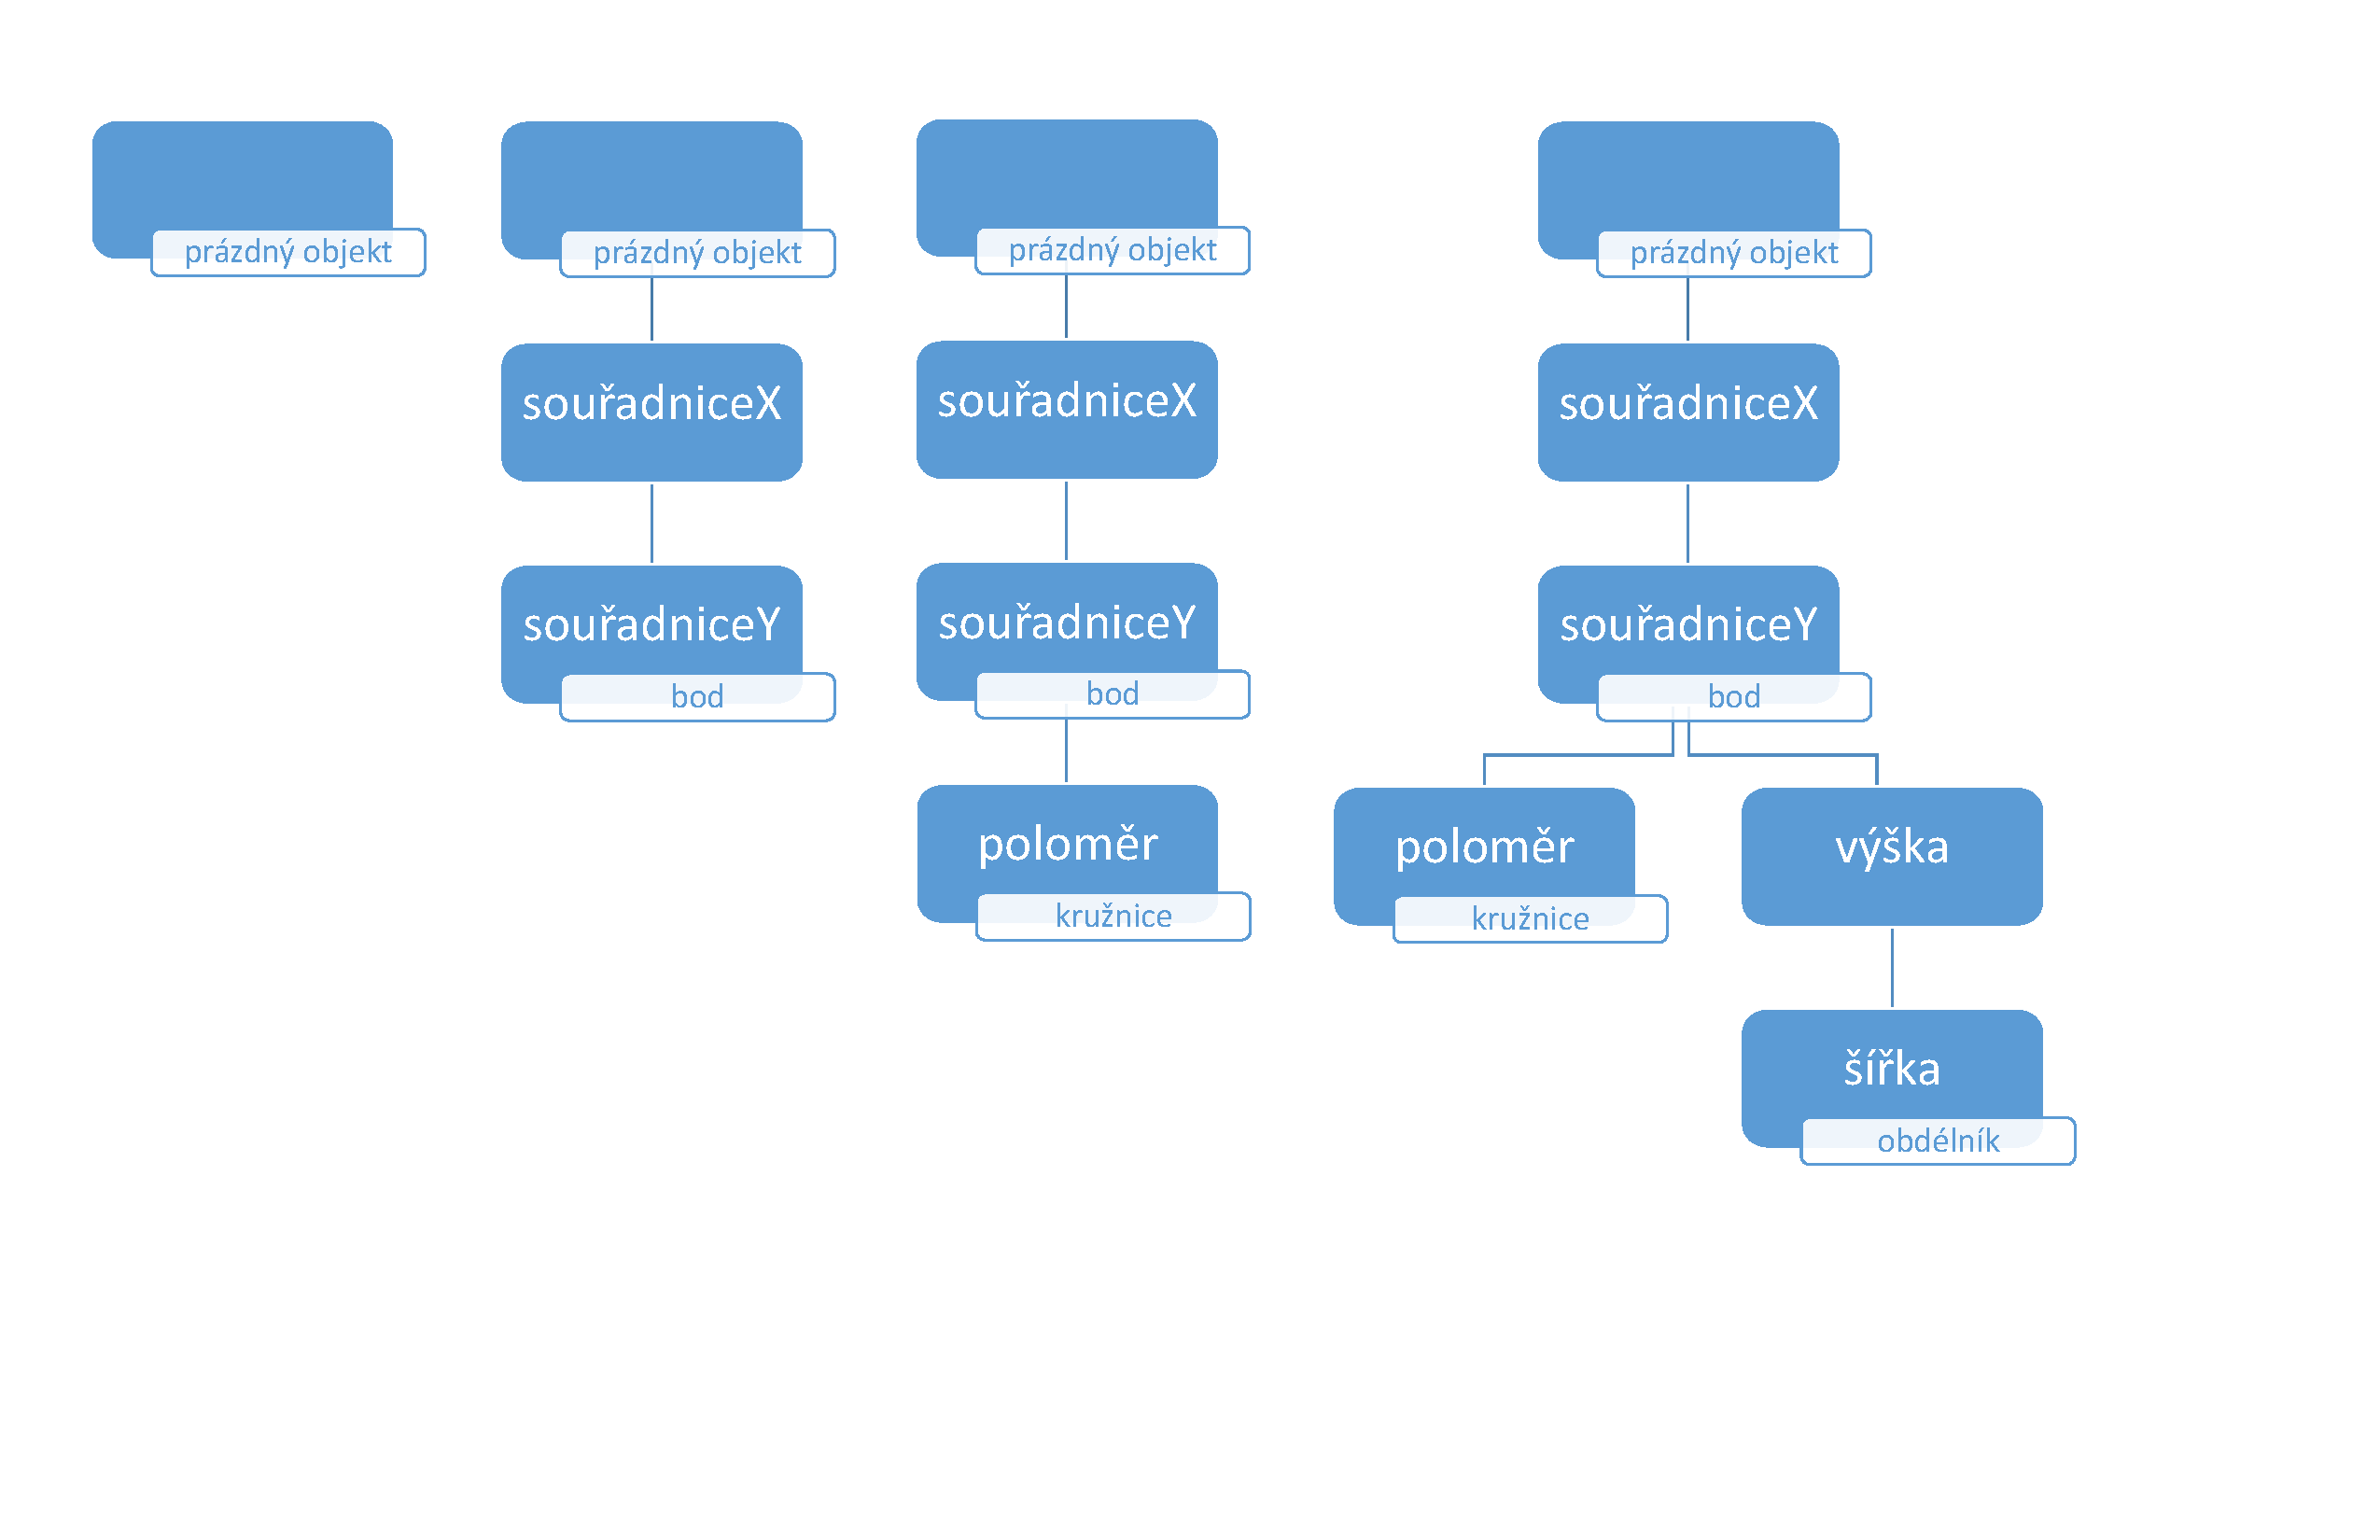
\includegraphics[trim=30 180 150 50, clip, angle=0, width=150mm]{cjsonStrom}
\caption{Postup vytvoření stromu šablon}
\label{cjsonKonstrukceStromu}
\end{figure}

\subsubsection{Vzorová data}
\textcolor{red}{Vytvořit data, popsat, upravit obrázek konstrukce stromu!!!}

Mějme homogenním poli zaměstnanců firmy, ve které máme uložené databázové id, příjmení a pozici, na které zaměstnanec pracuje. Tato kolekce může vypadat následujícím způsobem.

\texttt{[\\
\hspace*{5mm}\{ \textquotedblright id\textquotedblright : 1, \textquotedblright name\textquotedblright : \textquotedblright Sánchez\textquotedblright, \textquotedblright position\textquotedblright : \textquotedblright Manager\textquotedblright\ \},\\
\hspace*{5mm}\{ \textquotedblright id\textquotedblright : 2, \textquotedblright name\textquotedblright : \textquotedblright Duffy\textquotedblright, \textquotedblright position\textquotedblright : \textquotedblright Programmer\textquotedblright\ \},\\
\hspace*{5mm}\{ \textquotedblright id\textquotedblright : 3, \textquotedblright name\textquotedblright : \textquotedblright Tamburello\textquotedblright, \textquotedblright position\textquotedblright : \textquotedblright Worker\textquotedblright\ \}\\
]}

\subsubsection{Postup komprese}
\begin{enumerate}
\item Textová data jsou převedena na kolekci instancí tříd.
\item Ze všech instancí v kolekci jsou postupně vyzvednuty hodnoty a uloženy do kolekce objektů, které obsahují pouze kolekci příslušných hodnot, zároveň je konstruován strom šablon.
\item Ze stromu šablon je vytvořena kolekce šablon. Šablona je kolekce obsahující identifikátor šablony, ze které \uv{dědí}, a klíče. Identifikátor 0 je rezervován pro šablonu odpovídající prázdnému objektu.
\item Objekty s hodnotami jsou doplněny o identifikátor odpovídající šablony.
\item \label{cjsonItem0}Ze vzniklých kolekci vytvoříme objekt obsahující identifikátor kompresního algoritmu (klíč \texttt{"f"}), kolekce šablon (klíč \texttt{"t"}) a kolekce hodnot (klíč \texttt{"v"}) (viz Data po kompresi).
\item Objekt vzniklý v bodě \ref{cjsonItem0} serializujeme jako JSON do řetězce nebo souboru.
\end{enumerate}

\subsubsection{Data po kompresi}
\texttt{\{\hspace*{3mm}"f" : "cjson",\\
\hspace*{5mm}"t" : [ [ 0, "x", "y" ], [ 1, "width", "height" ] ],\\
\hspace*{5mm}"v" : [ \{ "" : [ 1, 100, 100 ] \}, \{ "" : [ 2, 100, 100, 200, 150 ] \} ] \}}

\subsubsection{Postup rekonstrukce dat}
\begin{enumerate}
\item Textová data jsou převedena na instanci třídy.
\item Vytvoříme kolekci, do které postupně vkládáme instance tříd vzniklé z prvků kolekce hodnot a příslušných šablon.
\item Tuto kolekci serializujeme jako JSON do řetězce nebo souboru.
\end{enumerate}